\section{Discussão dos Resultados Obtidos}

É objetivo desta seção apresentar e discutir os resultados obtidos a partir dos testes da técnica desenvolvida com o intuito de avaliar seu desempenho quanto a entrega de mensagens e seu consumo energético. Além disso, são discutidos os resultados obtidos quando a recarga das baterias é considerada com o intuito de analisar o comportamento a longo prazo.

Os resultados são apresentados na forma de gráficos, onde cada um deles são associados a uma das primeiras três letras do alfabeto, ou seja, as letras \emph{a}, \emph{b} e \emph{c}. A primeira delas é associada aos gráficos que apresentam o comportamento da rede quanto a probabilidade de entrega de mensagens; a segunda é combinada aos que exibem o comportamento quanto a quantidade de mensagens entregues aos destinatários; a última é relacionada a gráficos que apontam o comportamento médio da quantidade de energia armazenada nas baterias dos dispositivos. Cada um gráficos apresenta o comportamento da rede para cada um dos três protocolos testados e, simultaneamente, para os dois estados da técnica, ou seja, ligada (considerando o consumo dos dispositivos GPS) e desligada. 

\subsection{Desconsiderando Recarga Periódica}

Desconsiderar recargas periódicas permite analisar como a rede se comporta quanto ao consumo efetivo das baterias e entregas de mensagens em um curto período de tempo. Além disso, a visualização de pontos ideais de recarga é facilitada, permitindo testá-los e visualizar o comportamento da rede em longo prazo.

Nesta Subseção são apresentados e discutidos os resultados obtidos desconsiderando a recarga periódica das baterias para os dois períodos de busca propostos na Seção \ref{sec:cenario}, ou seja, 8, 32 e 56 segundos e 8, 32 e 32 segundos. referindo-se à ordem dos intervalos de cada combinação, sendo o mínimo, padrão e máximo, respectivamente.

\newpage
\subsubsection{Intervalo Busca de 8, 32 e 56 Segundos}
\label{8-32-56_semRecarga}

Quando se trata do intervalo de 8, 32 e 56 segundos, sendo o período de busca mínimo, padrão e máximo, respectivamente, a rede apresenta o comportamento apresentados nos gráficos da Figura \ref{10dias_8-32-56_semRecarga}.

É visto no gráfico \emph{c} que a técnica gera um maior consumo das baterias, o que se traduz na morte da rede por volta do final do sétimo dia de simulação. A falta de energia causa a interrupção na entrega de mensagens, como visto no gráfico \emph{b}, e, consequentemente a queda da probabilidade de entrega, apresentada no gráfico \emph{a}.

Pelos gráficos \emph{a} e \emph{b} é possível observar que, durante o tempo de atividade da rede a técnica não consegue se sobressair com relação a quantidade de mensagens entregues e, consequentemente, quanto a probabilidade de entrega. Isso, quando associado ao consumo adicional das baterias observado no gráfico \emph{c}, é entendido como um não aproveitamento da energia adicional consumida, pois não foi capaz de aumentar a quantidade de mensagens entregues.

A justificativa do consumo adicional das baterias é de simples argumentação. Ele se deve, primordialmente, ao consumo adicional gerado pelos dispositivos GPS, visto que, sem a técnica, estes dispositivos não são utilizados. Além disso, o consumo adicional gerado pela redução do intervalo de busca para até 8 segundos não é compensado pelo aumento até os 56 segundos.

Além disso, pode-se observar que os três protocolos apresentam uma linha de tendência semelhante. Todavia, é percebida uma ligeira vantagem do protocolo \emph{Prophet} em relação aos demais quanto a entrega de mensagens, gráfico \emph{b}, e a probabilidade de entrega, gráfico \emph{a}. Esse resultado permite observar a vantagem dos protocolos probabilísticos em relação aos não probabilísticos apresentada na Subseção \ref{subsec:encaminhamento_mensagens}.

Quando considerados os fatores apresentados, observa-se que a técnica não traz vantagens quando utilizada com os parâmetros definidos, visto que o consumo adicional das baterias não se traduziu no aumento da quantidade de mensagens entregues e, consequentemente, numa maior probabilidade de entrega de mensagens.

\begin{sidewaysfigure}
\centering
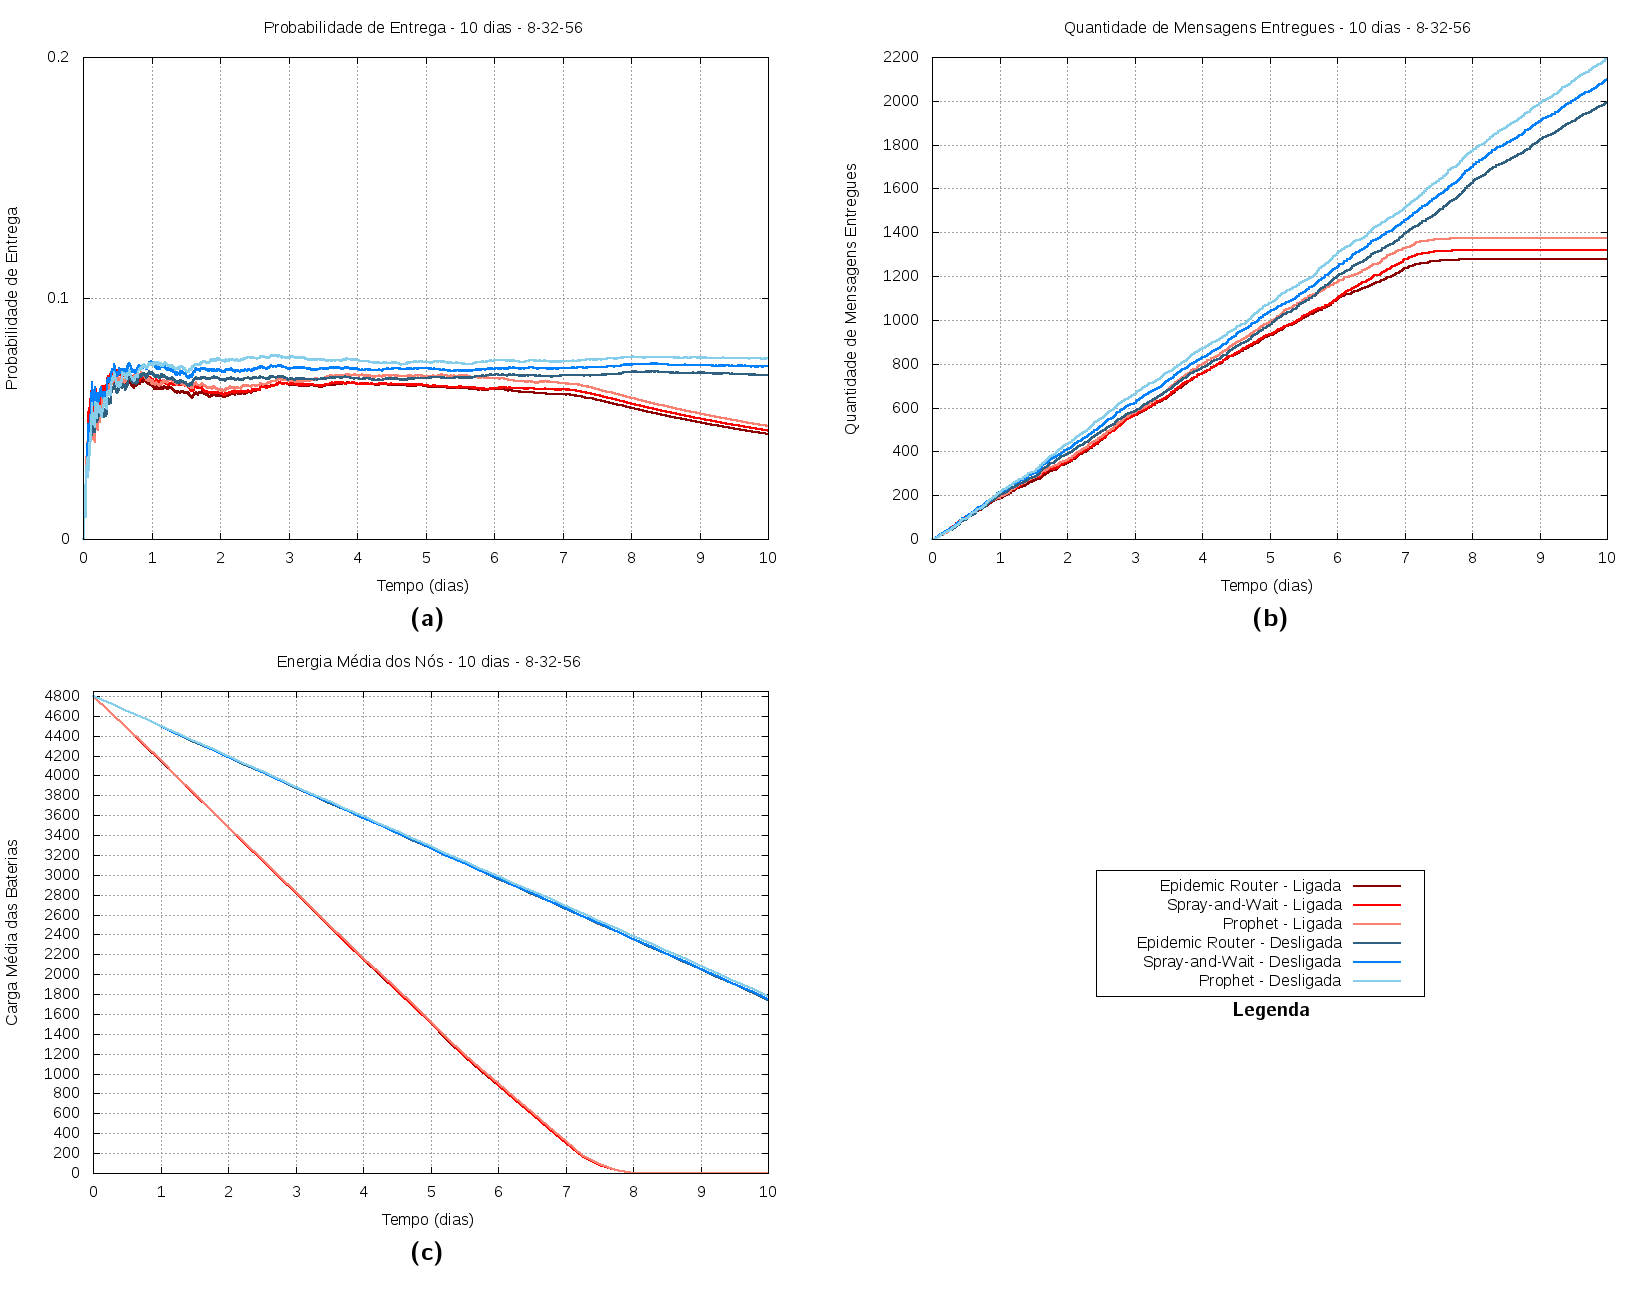
\includegraphics[width=0.8\textwidth]{figuras/cap_5/graficos/8_32_56/MessageDeliveryReport_10_8-32-56_noRecharge.png}
\caption{Resultados de simulações de 10 dias sem recarga periódica e período de busca de 8, 32 e 56 segundos.}
\label{10dias_8-32-56_semRecarga}
\end{sidewaysfigure}

\newpage
\subsubsection{Intervalo de Busca de 8, 32 e 32 Segundos}
\label{8-32-32_semRecarga}

Quando se trata do intervalo de 8, 32 e 32 segundos, sendo o período de busca mínimo, padrão e máximo, respectivamente, a rede apresenta o comportamento apresentados nos gráficos da Figura \ref{10dias_8-32-32_semRecarga}.

A redução do período de busca, que agora pode variar apenas dentro do intervalo de 8 a 32 segundos, acarretou num aumento significativo do consumo das baterias dos dispositivos, como visto no gráfico \emph{c}, reduzindo pela metade o tempo de vida da rede. Todavia, como visto nos gráficos \emph{a} e \emph{b}, a probabilidade de entrega e, consequentemente, a quantidade de mensagens entregues aumentaram significativamente durante o período de atividade da rede.

Os resultados obtidos quanto a quantidade de mensagens entregues durante o período de atividade da rede podem ser facilmente explicados. Eles são decorrentes da redução do período onde o intervalo de busca se situa, ou seja, de 8 a até 56 segundos para 8 a até 32 segundos, o que faz com que os dispositivos passem menos tempo aguardando por novos ciclos de busca, traduzindo-se numa maior quantidade de buscas por dispositivos. 

Aumentar a quantidade de buscas por outros dispositivos resulta num aumento da quantidade tempo que os dispositivos passam buscando por outros. Consequentemente, contatos que antes seriam perdidos devido aos dispositivos estarem aguardando por outro ciclo de busca ocorrem com menor frequência. Finalmente, há uma maior quantidade de oportunidades de contato, o que resulta num aumento da quantidade de mensagens entregues e na probabilidade de entrega de mensagens durante o período de atividade da rede.

O ajuste dinâmico, provido pela técnica a partir do uso das tabelas de mapeamento, garante que os intervalos entre as buscas fiquem menores em regiões com alta probabilidade de contato, aumentando ainda mais a quantidade deles devido ao melhor aproveitamento das baterias em situações onde aumentar o consumo é uma decisão inteligente.

Em decorrência da maior quantidade de mensagens entregues, durante o período de atividade da rede, a probabilidade de entrega se manteve acima da rede que não utiliza a técnica. Ao interromper suas atividades por falta de energia, a rede não entrega mais mensagens e, como consequência, a probabilidade de entrega cai gradativamente até que esta fique menor que a da rede que não utiliza a técnica desenvolvida.

A morte prematura da rede torna ineficiente a utilização da técnica quando não é considerada a recarga das baterias dentro do cenário analisado. Todavia, a vantagem da técnica durante o período de atividade da rede pode ser melhor explorada quando é considerada a recarga.

\begin{sidewaysfigure}
\centering
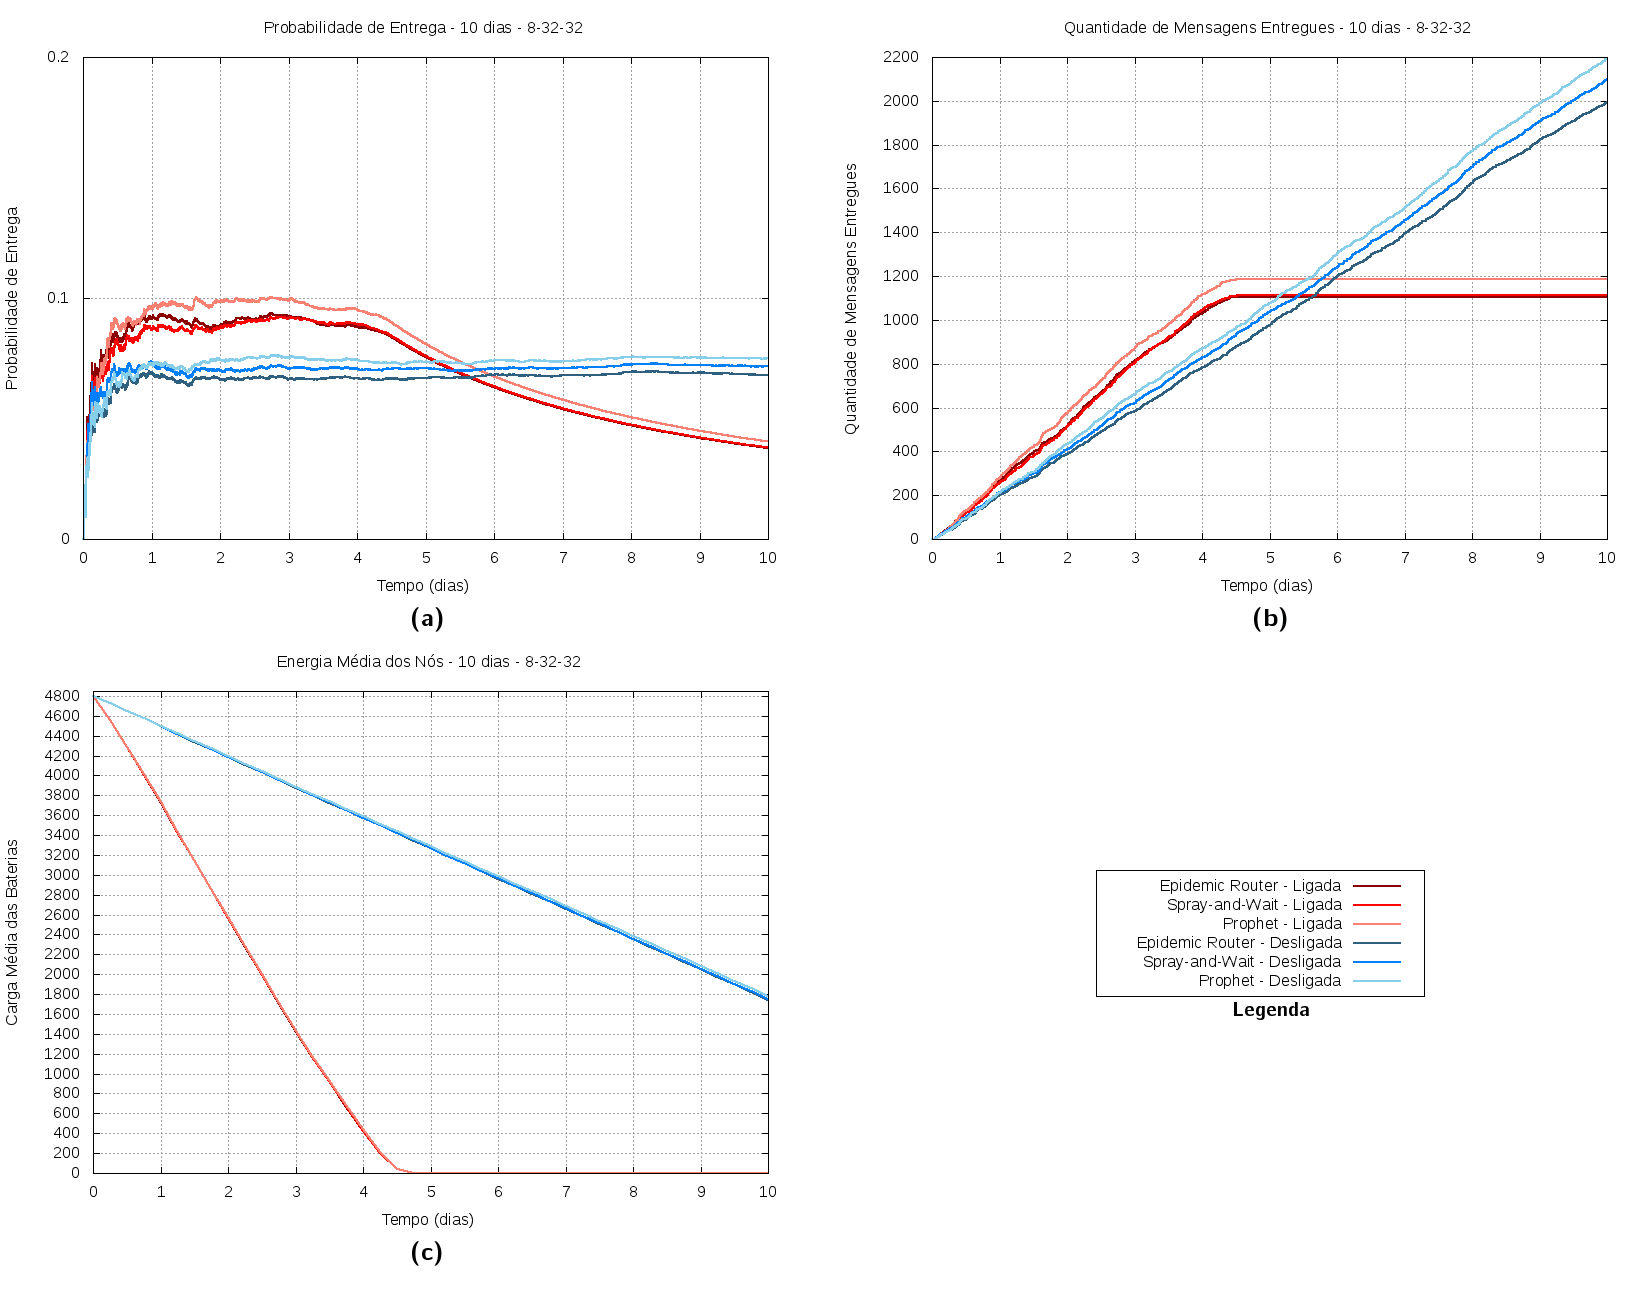
\includegraphics[width=0.8\textwidth]{figuras/cap_5/graficos/8_32_32/MessageDeliveryReport_10_8-32-32_noRecharge.png}
\caption{Resultados de simulações de 10 dias sem recarga periódica e período de busca de 8, 32 e 32 segundos.}
\label{10dias_8-32-32_semRecarga}
\end{sidewaysfigure}

\subsubsection{Discussões Sobre o Cenário sem Recarga das Baterias}

Dentro dos intervalos testados, o que apresentou pior desempenho foi o de 8, 32 e 56 segundos. Este resultado é decorrente da ineficiência quanto ao consumo adicional gerado pela técnica devido ao uso de dispositivos GPS e a quantidade inferior de mensagens entregues ao ser comparada com uma DTN que não a utiliza. Quando a linha de tendência dos gráficos da Figura \ref{10dias_8-32-56_semRecarga} é analisada, é possível concluir que durante o tempo de vida da rede, mesmo quando realizadas recargas, não ocorrerão melhorias quanto a quantidade de mensagens entregues. Essa situação é verificada logo a seguir.

O intervalo de 8, 32 e 32 segundos apresentou um desempenho consideravelmente melhor quanto a probabilidade de entrega e quantidade de mensagens entregues durante o tempo de vida da rede. Esse resultado é proveniente do consumo inteligente das baterias atrelado a redução do período que o intervalo de busca se situa. Quando analisa-se linha de tendência da quantidade de mensagens entregues, percebe-se que, durante o tempo de atividade da rede, a técnica apresenta vantagens e estas podem ser aproveitadas quando a recarga das baterias é considerada. Esta situação será verificada na Subseção \ref{subsec:testes_com_recarga}.

Analisando a fundo o consumo adicional de energia gerado pela técnica, é percebido que quanto menor for o intervalo de busca ideal de uma região, maior é o consumo de energia. Isso se deve ao fato de que uma consulta GPS precisa ser realizada quando os dispositivos precisam calcular o novo período de espera, como apresentado na Subseção \ref{sec:dinamizacao_intervalo_busca}. Além disso, quanto menor esse período, maior a quantidade de buscas e, consequentemente, maior ainda a energia consumida por esses componentes.

Finalmente, quando considerado um cenário onde não existe a possibilidade de recarga das baterias, a técnica apresenta desvantagem, visto que os testes indicaram a morte prematura da rede quando ela é utilizada.

\subsection{Considerando Recarga Periódica}
\label{subsec:testes_com_recarga}

Dentro do âmbito das DTNs, a recarga periódica de baterias é possível em diversos cenários, exemplificando-se com o uso de placas solares em situações como as aplicações espaciais e o projeto ZebraNet \cite{zhang2004hardware}. Além disso, considerar a recargadas baterias permite analisar o comportamento da técnica a longo prazo.

Nesta Subseção são apresentados e discutidos os resultados obtidos considerando a recarga periódica das baterias para os dois períodos de busca propostos na Subseção \ref{sec:cenario}, ou seja, 8, 32 e 56 segundos e 8, 32 e 32 segundos, sendo os intervalos mínimo, padrão e máximo, respectivamente.

\subsubsection{Intervalo de Busca de 8, 32 e 56 Segundos}
\label{8-32-56_comRecarga}

A partir da análise do gráfico \emph{c} da Figura \ref{10dias_8-32-56_semRecarga}, conclui-se que todos os dispositivos da rede têm suas baterias esgotadas ao final do sétimo dia. Partindo disso pode-se definir um intervalo máximo de recarga no exato ponto onde a rede encerra a sua atividade para analisar o seu comportamento a longo prazo.

Num cenário de 10 dias de simulação e com um período de recarga de sete dias, foi observado o comportamento dos gráficos da Figura \ref{10dias_8-32-56_comRecarga}. No gráfico \emph{a} pode ser visto que a probabilidade de entrega da técnica encontra-se abaixo em relação a uma rede que não a utiliza. A probabilidade de entrega é refletida na quantidade de mensagens entregues que, por sua vez, também apresenta desvantagem, como visto no gráfico \emph{b} da mesma Figura. Pode ser observado que os resultados estão de acordo com a linha de tendência observada nos resultados apresentados na Figura \ref{10dias_8-32-56_semRecarga} durante o tempo de atividade da rede simulada.

A longo prazo, num período de 30 dias, a rede apresenta o comportamento visto na Figura \ref{30dias_8-32-56_comRecarga}, onde pode ser observada a mesma linha de tendência da Figura \ref{10dias_8-32-56_comRecarga}, tanto para a probabilidade de entrega quanto para a quantidade de mensagens entregues. A probabilidade de entrega utilizando a técnica, apresentada no gráfico \emph{a}, se mantém estável porém abaixo da rede que não a utiliza. O gráfico \emph{b} reflete a situação do gráfico \emph{a}, onde a quantidade de mensagens entregues também se mantém abaixo de uma rede sem a técnica. Com a técnica 5706 mensagens foram entregues contra 6170 mensagens sem ela, ou seja, uma diferença de 464 mensagens. Todos os valores referem-se as quantidades médias dos dados observados.

\begin{sidewaysfigure}
\centering
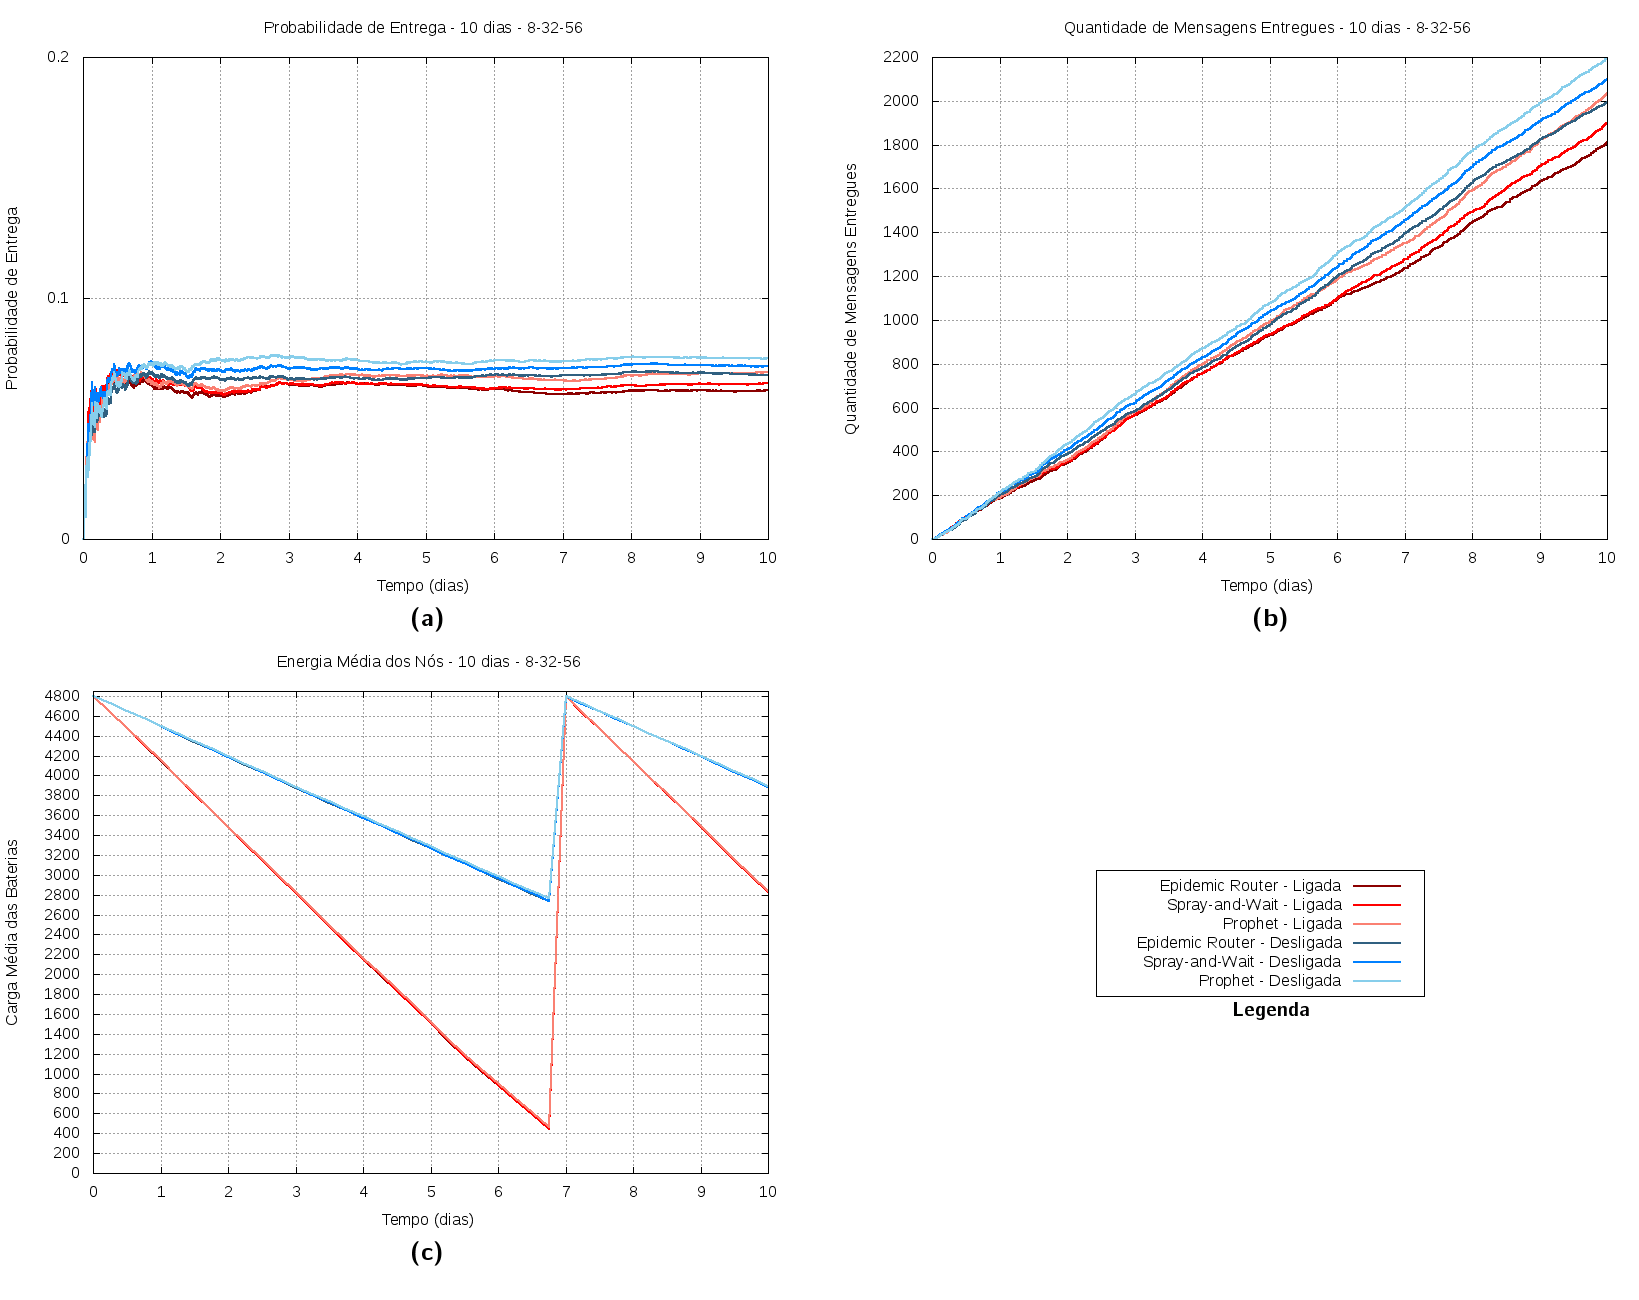
\includegraphics[width=0.8\textwidth]{figuras/cap_5/graficos/8_32_56/MessageDeliveryReport_10_8-32-56_withRecharge_604800.png}
\caption{Resultados de simulações de 10 dias com recarga periódica de sete dias e período de busca de 8, 32 e 56 segundos.}
\label{10dias_8-32-56_comRecarga}
\end{sidewaysfigure}

\begin{sidewaysfigure}
\centering
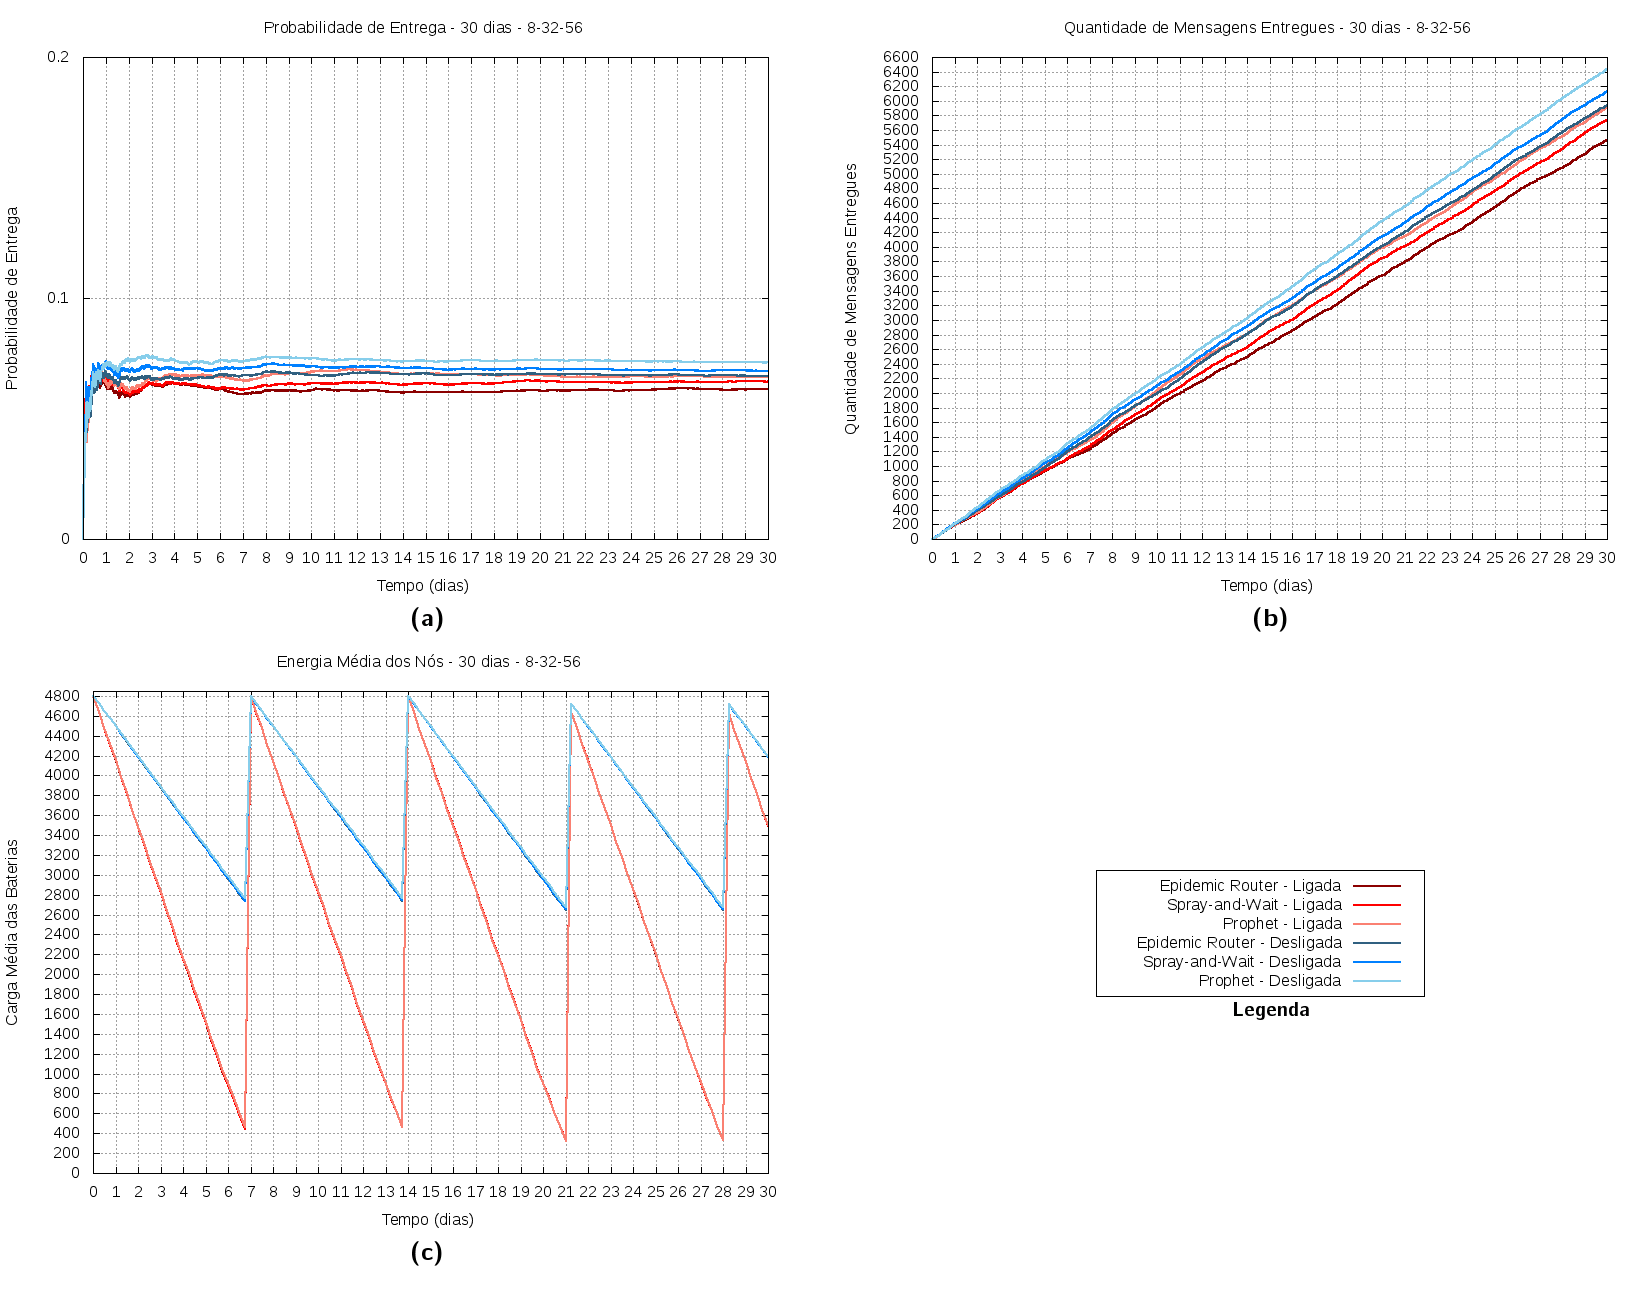
\includegraphics[width=0.8\textwidth]{figuras/cap_5/graficos/8_32_56/MessageDeliveryReport_30_8-32-56_withRecharge_604800.png}
\caption{Resultados de simulações de 30 dias com recarga periódica de sete dias e período de busca de 8, 32 e 56 segundos.}
\label{30dias_8-32-56_comRecarga}
\end{sidewaysfigure}

Quando analisado o consumo de energia, o comportamento dos gráficos \emph{c} das Figuras \ref{10dias_8-32-56_comRecarga} e \ref{30dias_8-32-56_comRecarga} é semelhante, visto que as redes utilizam os mesmos parâmetros de simulação, diferindo apenas na quantidade de tempo considerada. A técnica visivelmente gera um consumo expressivo das baterias que, neste cenário, não é bem aproveitado quando considerada a quantidade de mensagens entregues e a probabilidade de entrega de mensagens.

\subsubsection{Intervalo de Busca de 8, 32 e 32 Segundos}
\label{8-32-32_comRecarga}

O desempenho satisfatório quanto a entrega de mensagens durante o tempo de atividade da rede visto apresentado nos resultados testes da Figura \ref{10dias_8-32-32_semRecarga} pode ser explorado quando a recarga das baterias é considerada, pois a rede encerrou a sua atividade pela escassez de recursos energéticos.

Intuitivamente, pode-se considerar que o ponto ideal de recarga localiza-se no instante de tempo onde as linhas da probabilidade de entrega se cruzam, pois é nesse momento que a técnica começa a apresentar desvantagem em relação a sua não utilização. Tal ponto está no início do quinto dia e este é utilizado como parâmetro na simulação representada pela Figura \ref{10dias_8-32-32_comRecarga_450000} como intervalo de recarga.

\begin{sidewaysfigure}
\centering
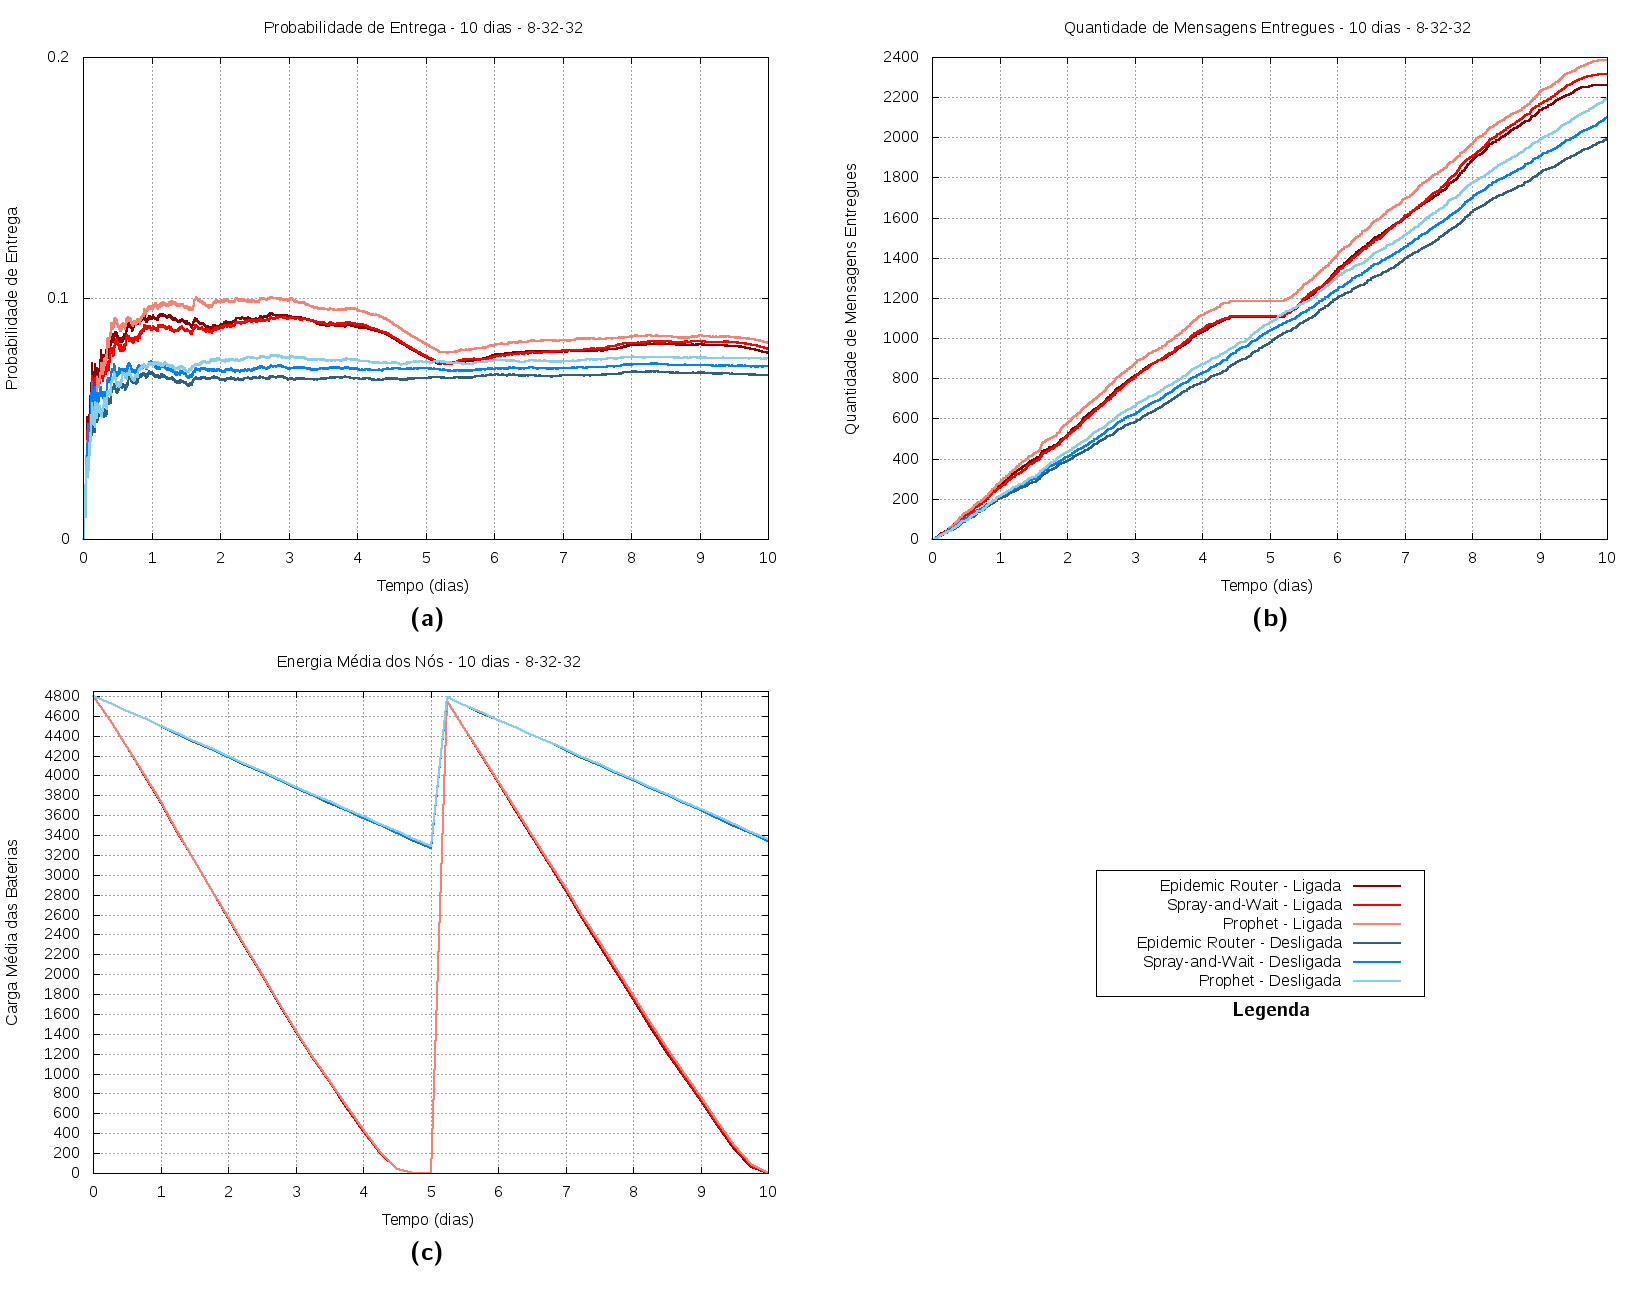
\includegraphics[width=0.8\textwidth]{figuras/cap_5/graficos/8_32_32/MessageDeliveryReport_10_8-32-32_withRecharge_450000.png}
\caption{Resultados de simulações de 10 dias com recarga periódica de cinco dias e período de busca de 8, 32 e 32 segundos.}
\label{10dias_8-32-32_comRecarga_450000}
\end{sidewaysfigure}

Os resultados, entretanto, demonstram que recarregar as baterias no período proposto não é vantajoso. Como pode ser visto no gráfico \emph{c}, a rede interrompe a sua operação por falta de energia por volta da metade do quarto dia, entretanto a recarga das baterias só é realizada 12 horas depois. A inatividade da rede resulta na interrupção da entrega de mensagens, como visto no gráfico \emph{b}, e, consequentemente, na diminuição da probabilidade de entrega, como apresentado no gráfico \emph{a}. Após a recarga das baterias a rede volta a entregar mensagens, porém a probabilidade de entrega não retorna ao valor que estava antes das baterias esgotarem suas cargas.

Recarregar as baterias de cinco em cinco dias não aproveita totalmente o potencial que a técnica possui quanto a entrega de mensagens, pois muitas oportunidades de contato são perdidas durante o período de inatividade da rede. A técnica, no entanto, apresentou um desempenho superior a uma rede que não a utiliza, visto que foi capaz de entregar 2320 mensagens contra 2097 mensagens, ou seja, uma diferença de 223 mensagens a mais. Todos os valores referem-se às médias de mensagens entregues no período simulado.

\newpage
Tendo em vista os resultados da Figura \ref{10dias_8-32-32_comRecarga_450000}, um período de recarga de quatro dias foi proposto e os resultados das simulações são apresentados na Figura \ref{10dias_8-32-32_comRecarga_345600}. Pode ser visto no gráfico \emph{b} da Figura \ref{10dias_8-32-32_comRecarga_345600} que a técnica obteve um melhor aproveitamento quanto a quantidade de mensagens entregues e que, por sua vez, refletiu na probabilidade de entrega que se manteve praticamente constante e acima da rede que não a utiliza após a sua estabilização ao final do terceiro dia.

\begin{sidewaysfigure}
\centering
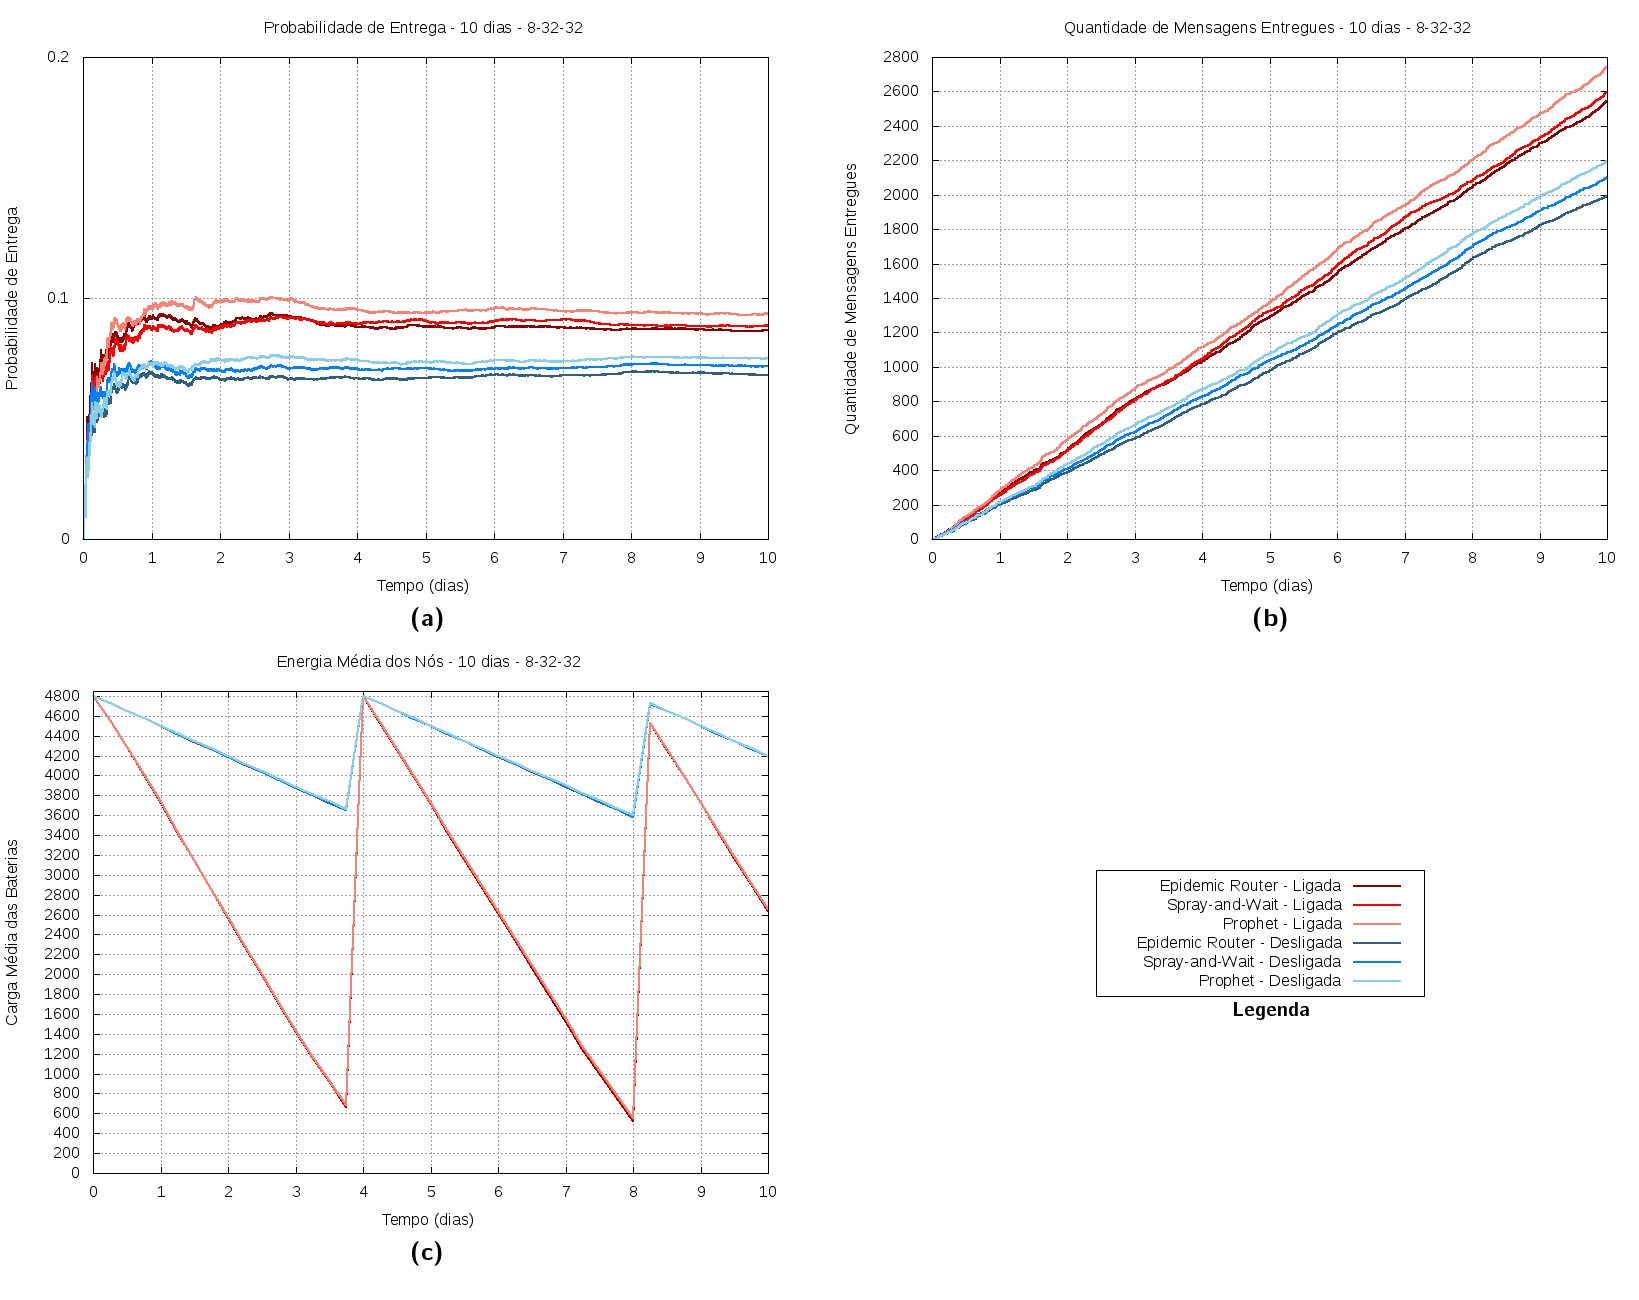
\includegraphics[width=0.8\textwidth]{figuras/cap_5/graficos/8_32_32/MessageDeliveryReport_10_8-32-32_withRecharge_345600.png}
\caption{Resultados de simulações de 10 dias com recarga periódica de quatro dias e período de busca de 8, 32 e 32 segundos.}
\label{10dias_8-32-32_comRecarga_345600}
\end{sidewaysfigure}

Ainda do contexto dos resultados apresentados na Figura \ref{10dias_8-32-32_comRecarga_345600}, a rede que utiliza o intervalo fixo de 32 segundos foi capaz de entregar 2096 mensagens contra 2627 mensagens da rede que utiliza a técnica desenvolvida, ou seja, uma diferença de 531 mensagens. Todos os valores se referem as médias dos resultados observados.

Quando analisada num período de 30 dias, foram obtidos os resultados apresentados na Figura \ref{30dias_8-32-32_comRecarga_345600}, onde é percebido um aumento na diferença de quantidade de mensagens entregues. Em números, a técnica desenvolvida foi capaz de entregar 7832 mensagens contra 6170 mensagens por uma rede com intervalo de busca fixo em 32 segundos. Ou seja, a média de mensagens entregues subiu de 531 para 1662. Novamente, todos os valores referem-se as médias dos resultados observados. A probabilidade de entrega, como consequência do maior número de mensagens entregues, também permaneceu acima de uma rede que não faz uso da técnica desenvolvida.

\begin{sidewaysfigure}
\centering
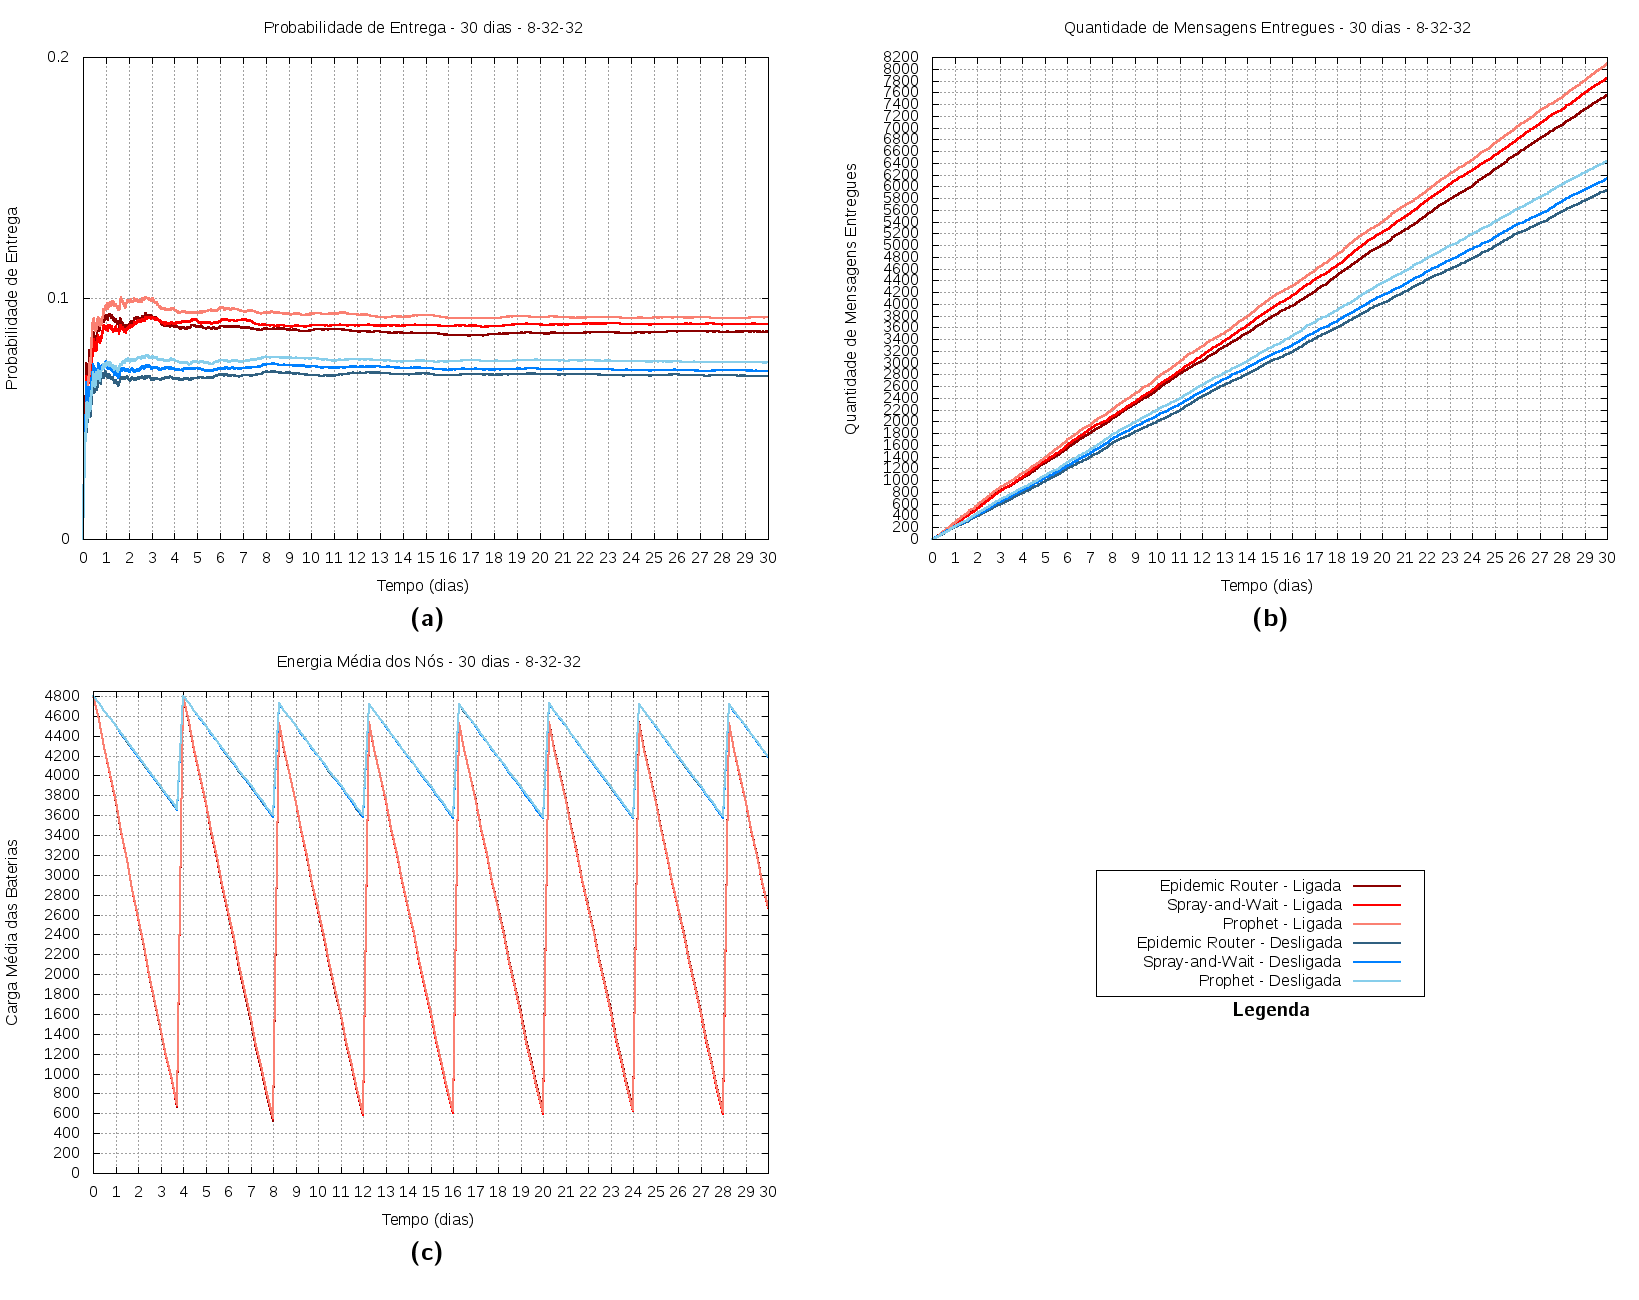
\includegraphics[width=0.8\textwidth]{figuras/cap_5/graficos/8_32_32/MessageDeliveryReport_30_8-32-32_withRecharge_345600.png}
\caption{Resultados de simulações de 30 dias com recarga periódica de quatro dias e período de busca de 8, 32 e 32 segundos.}
\label{30dias_8-32-32_comRecarga_345600}
\end{sidewaysfigure}

\subsubsection{Discussões Sobre o Cenário com Recarga das Baterias}

A ineficiência da técnica quanto ao intervalo de 8, 32 e 56 segundos foi novamente observada, desta vez em um cenário onde a recarga das baterias foi considerada. A quantidade inferior de mensagens entregues e, consequentemente, a menor probabilidade de entrega em relação a sua não utilização torna ineficiente o uso da técnica com os parâmetros definidos, visto que ela não foi capaz de compensar o consumo adicional das baterias em prol da entrega de mensagens.

O intervalo de 8, 32 e 32 segundos, entretanto, apresentou um desempenho melhor quando analisada a probabilidade de entrega e a quantidade de mensagens entregues. Num cenário de simulação de 30 dias, em média, a técnica foi capaz de entregar de 7832 mensagens contra 6170 mensagens entregues por uma rede que baseia-se no período fixo de 32 segundos. A diferença positiva de 1662 mensagens entregues pela técnica é considerável e, quanto maior o tempo de atividade da rede, maior será este valor.

O consumo adicional de energia gerado pela técnica, no caso do intervalo de 8, 32 e 32 segundos, traduziu-se numa maior quantidade de mensagens entregues. Evidenciando assim que tornar inteligente o consumo das baterias não significa, necessariamente, poupá-las.

Discussões sobre o ponto ótimo de recarga devem ser realizadas. Neste trabalho foi evidenciado, por meio dos resultados apresentados nas Figuras \ref{10dias_8-32-32_comRecarga_450000} e \ref{10dias_8-32-32_comRecarga_345600}, que o período de recarga precisa, necessariamente, ser no máximo o tempo de vida da rede implementada para que a técnica tenha melhor aproveitamento quanto a quantidade de mensagens entregues. Isso se deve ao fato de que, caso o período seja maior que o tempo máximo que a rede consegue ficar ativa, os dispositivos irão ficar inativos repetidamente e, como consequência, diversas oportunidades de contato serão perdidas e interrupções na entrega de mensagens serão observadas.
